\section{Support vector machine}\label{sec:SVMintro}% and the relation with Binary Logistic Regression}
There is a lot of work about SVM in literature , see \cite{drucker1997support,ben2001support,cortes1995support,cristianini2000introduction} for example.
Given a binary linearly separable classification dataset ${(x_i,y_i)}_{i = 1}^N$, where $x_i\in \mathbb{R}^d, y_i\in \left \{\begin{pmatrix}1\\0\end{pmatrix}, \begin{pmatrix}0\\1\end{pmatrix}\right \}$. We use $A_1,A_2$ to denote the data with label $\begin{pmatrix}1\\0\end{pmatrix}, \begin{pmatrix}0\\1\end{pmatrix}$, respectively. Our goal is to find a $\theta = (w,b)$ where $w\in \mathbb{R}^{1\times d}, b\in \mathbb{R}$ such that the hyperplane $H_{\theta} = \{x:wx + b = 0\}$ can separate $A_1,A_2$.

\subsection{Binary SVM}\label{sec:SVM}
Binary Support Vector Machine (SVM for short hereinafter) wants to find the classifiable hyperplane which has the biggest distance with $A_1$ and $A_2$. Assume that we have the hyperplanes $wx+b=\pm 1$ with
$$
wx_i+b\ge 1 \quad \mbox{for}\quad x_i\in A_1,\quad wx_i+b\le -1 \quad \mbox{for}\quad x_i\in A_2,
$$
which is similar to the definition \eqref{2classH}.
Let $y_1=\begin{pmatrix}1\\0\end{pmatrix}$ for $x_i\in A_1$ and $y_2=\begin{pmatrix}0\\1\end{pmatrix}$ for $x_i\in A_2$. %Then, we have the following inequality
%$$
%y_i(wx_i+b)\ge 1 \quad \mbox{for all }\quad i.
%$$
Note that $w$ is normal to the hyperplane and the distance  between the points satisfying 
$$
wx_i+b=\pm 1
$$
and the hyperplane $wx+b=0$ is $\displaystyle {1\over \|w\|_2}$. Thus, the width of the margin is $\displaystyle {2\over \|w\|_2}$ as shown in Figure \ref{fig:margin}.
\begin{figure}
	\centering
	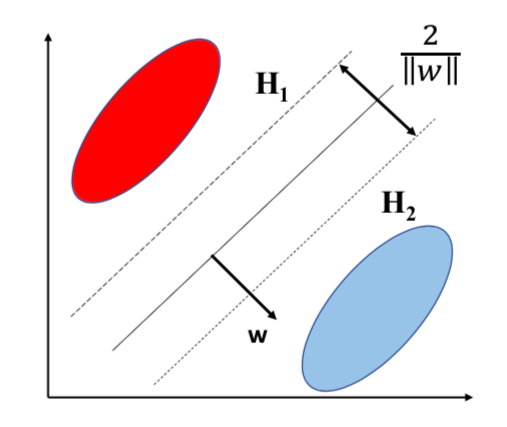
\includegraphics[width = 2in]{margin}
	\caption{SVM}
	\label{fig:margin}
\end{figure}
For any $w$ and $b$, the smallest distance between points and the hyperplane is 
\begin{equation}
\frac{\min_{i} \ell_i(wx_i+b)}{\|w\|_2},
\end{equation} 
where $\ell_i=1-2e_2^Ty_i$.
Note that 
$$
\ell_i=\begin{cases}
1 & \mbox{ if } y_i=\begin{pmatrix}1\\0\end{pmatrix},
\\
-1 &\mbox{ if } y_i=\begin{pmatrix}0\\1\end{pmatrix}.
\end{cases}
$$
Consider the problem
\begin{equation}
	\max_{w,b} \frac{\min_{i} \ell_i(wx_i+b)}{\|w\|_2}.
\end{equation}
Intuitively, the best separating hyperplane $H$ is only determined by those data points who are closest to $H$. Those data points are called {support vector}, and this method are called {support vector machine}.

Without loss of generality, we may restrict the norm of $\|w\|$ to be 1, which leads to a equivalent optimization problem
\begin{equation}
\max_{\|w\|_2 = 1} \min_{i} \ell_i(wx_i+b)
\end{equation}
Actually, {we can prove $\displaystyle \mathop{\rm argmax}_{\|w\|_2 = 1} \min_{i} \ell_i(wx_i+b)$ is nonempty, but here we just admit this fact and only prove the uniqueness of the solution.}

\begin{lemma}
	If $A_1,A_2$ are linearly separable, then
	\begin{equation}\label{binarySVM}
	\mathop{\rm argmax}_{\|w\|_2 = 1} \min_{i} \ell_i(wx_i+b)
	\end{equation}
	is nonempty.
\end{lemma}

\begin{proof}
	Take $x_{i_1} \in A_1$ and  $x_{i_2} \in A_2$,  given $(w,b)\in \{(w,b): l_i(wx_i +b)>0, \forall i\}$, we have
	\begin{equation}
		\begin{cases}
		wx_{i_1} + b > 0,\\
		wx_{i_2} + b < 0
		\end{cases}
	\end{equation}
	which implies $|b| < \max_{i} \|x_i\|_2$. So we have
	\begin{equation}
		\mathop{\rm argmax}_{\|w\|_2 = 1} \min_{i} \ell_i(wx_i+b) = \mathop{\rm argmax}_{\|w\|_2 = 1, ~|b|\leq \max_{i} \|x_i\|_2} \min_{i} \ell_i(wx_i+b) \neq \emptyset.
	\end{equation}
\end{proof}

\begin{lemma}
	If $A_1,A_2$ are linearly separable, then
	\begin{equation}
		\mathop{\rm argmax}_{\|w\|_2 = 1} \min_{i} \ell_i(wx_i+b)
	\end{equation}
	 is a singleton set.
\end{lemma}

\begin{proof}
	Denote $\displaystyle m(w,b) = \min_{i} \ell_i(wx_i+b)$. Notice that $m(w,b)$ is a concave homogeneous function w.r.t $w,b$ and $\|\cdot\|_2$ is a strictly convex norm. Suppose there are two solution $(w_1,b_1)$ and $(w_2,b_2)$ such that $w_1 \neq w_2$, take $\overline{w} = \frac{w_1 + w_2}{2}, \overline{b} = \frac{b_1 + b_2}{2}$, we must have
	\begin{equation}
		m(\overline{w},\overline{b}) \geq \frac{m(w_1,b_1)+ m(w_2,b_2)}{2} = \max_{\|w\|_2 = 1} m(w,b),
	\end{equation}
	and 
	\begin{equation}
		\|\overline{w}\|_2 < 1.
	\end{equation}
	So
	\begin{equation}
		m(\frac{\overline{w}}{\|\overline{w}\|_2},\frac{\overline{b}}{\|\overline{w}\|_2}) = \frac{m(\overline{w},\overline{b}) }{\|\overline{w}\|_2} > \max_{\|w\|_2 = 1} m(w,b),
	\end{equation}
	which leads to a contradiction. So all the solutions must have the same $w$, we denote it as $w^*$. Then if $(w^*,b^*)$ is a solution of problem (\ref{binarySVM}), we must have
	\begin{equation}
		b^* \in \mathop{\rm argmax}_{b} m(w^*,b)
	\end{equation}
	Actually,
	\begin{equation}
		m(w^*,b) = \min\{b+\min_{x\in A_1} w^*x, -b +\min_{x\in A_2} (-w^*x)\}.
	\end{equation}
	It is easy to observe that $\displaystyle \mathop{\rm argmax}_{b} m(w^*,b)$ is a singleton set and 
	\begin{equation}
		b^* = \frac{\min_{x\in A_2} (-w^*x) - \min_{x\in A_1} w^*x}{2}.
	\end{equation}
\end{proof}

Denote
\begin{equation}\label{maxSVM}
	\theta^*_{SVM} = (w_{SVM}^*,b_{SVM}^*) = \mathop{\rm argmax}_{\|w\|_2 = 1} \min_{i} \ell_i(wx_i+b).
\end{equation}


\begin{theorem}[Representation Theorem]
	Let $\theta^*_{SVM} = (w_{SVM}^*,b_{SVM}^*) $ be the solution of \eqref{maxSVM}. Then, $w_{SVM}^*$ must be a linear combination of $x_i^T, i = 1,2,\cdots,N$.
\end{theorem}

\begin{proof}
	Denote
	\begin{equation}
		S = {\rm span} \{x_i^T\}_{i=1}^N.
	\end{equation}
	Then we have
	\begin{equation}
		\mathbb{R}^{1\times d} = S \oplus^{\perp} S^{\perp}.
	\end{equation}
	So $w_{SVM}^*$ can be uniquely decomposed as $w_{SVM}^* = w^*_S + w^*_{S^{\perp}}$ where $w_S\in S$ and $w^*_{S^{\perp}}\in S^{\perp}$. 
	We will prove that $w^*_{S^{\perp}} = 0$. Suppose not, we have
	\begin{equation}
		\|w^*_S\|_2 < \|w_{SVM}^*\|_2 = 1. 
	\end{equation}
	Notice that
	\begin{equation}
		w_{SVM}^* x_i = w_S^* x_i,\ \forall i = 1,2,\cdots,N.
	\end{equation}
	Thus we have
	\begin{equation}
		\min_{i} \ell_i(w_{SVM}^*x_i+b_{SVM}^*) = \min_{i} \ell_i(w_S^*x_i+b_{SVM}^*).
	\end{equation}
	So
	\begin{equation}
	\min_{i} \ell_i(w_{SVM}^*x_i+b_{SVM}^*) < \frac{\min_{i} \ell_i(w_S^*x_i+b_{SVM}^*)}{\|w_S^*\|} = \min_{i} \ell_i(\frac{w^*_S}{\|w_S^*\|_2}x_i+\frac{b_{SVM}^*}{\|w^*_S}\|_2),
	\end{equation}
	which leads to a contradiction to the definition of $\theta_{SVM}^*$.
\end{proof}

%For any $w$ and $b$, the smallest distance between points and the hyperplane is 
%\begin{equation}
%\frac{\min_{i} y_i(wx_i+b)}{\|w\|_2}.
%\end{equation} Consider the problem
%\begin{equation}
%	\max_{w,b} \frac{\min_{i} y_i(wx_i+b)}{\|w\|_2}.
%\end{equation}
%Intuitively, the best separating hyperplane $H$ is only determined by those data points who are closest to $H$. Those data points are called {support vector}, and this method are called {support vector machine}.
%
%Without loss of generality, we may restrict the norm of $\|w\|$ to be 1, which leads to a equivalent optimization problem
%\begin{equation}
%\max_{\|w\|_2 = 1} \min_{i} y_i(wx_i+b)
%\end{equation}
%Actually, {we can prove $\displaystyle \mathop{\rm argmax}_{\|w\|_2 = 1} \min_{i} y_i(wx_i+b)$ is nonempty, but here we just admit this fact and only prove the uniqueness of the solution.}
%
%\begin{lemma}
%	If $A_1,A_2$ are linearly separable, then
%	\begin{equation}\label{binarySVM}
%		\mathop{\rm argmax}_{\|w\|_2 = 1} \min_{i} y_i(wx_i+b)
%	\end{equation}
%	 is a singleton set.
%\end{lemma}
%
%\begin{proof}
%	Denote $\displaystyle m(w,b) = \min_{i} y_i(wx_i+b)$. Notice that $m(w,b)$ is a concave homogeneous function w.r.t $w,b$ and $\|\cdot\|_2$ is a strictly convex norm. Suppose there are two solution $(w_1,b_1)$ and $(w_2,b_2)$ such that $w_1 \neq w_2$, take $\overline{w} = \frac{w_1 + w_2}{2}, \overline{b} = \frac{b_1 + b_2}{2}$, we must have
%	\begin{equation}
%		m(\overline{w},\overline{b}) \geq \frac{m(w_1,b_1)+ m(w_2,b_2)}{2} = \max_{\|w\|_2 = 1} m(w,b),
%	\end{equation}
%	and 
%	\begin{equation}
%		\|\overline{w}\|_2 < 1.
%	\end{equation}
%	So
%	\begin{equation}
%		m(\frac{\overline{w}}{\|\overline{w}\|_2},\frac{\overline{b}}{\|\overline{w}\|_2}) = \frac{m(\overline{w},\overline{b}) }{\|\overline{w}\|_2} > \max_{\|w\|_2 = 1} m(w,b),
%	\end{equation}
%	which leads to a contradiction. So all the solutions must have the same $w$, we denote it as $w^*$. Then if $(w^*,b^*)$ is a solution of problem (\ref{binarySVM}), we must have
%	\begin{equation}
%		b^* \in \mathop{\rm argmax}_{b} m(w^*,b)
%	\end{equation}
%	Actually,
%	\begin{equation}
%		m(w^*,b) = \min\{b+\min_{x\in A_1} w^*x, -b +\min_{x\in A_2} (-w^*x)\}.
%	\end{equation}
%	It is easy to observe that $\displaystyle \mathop{\rm argmax}_{b} m(w^*,b)$ is a singleton set and 
%	\begin{equation}
%		b^* = \frac{\min_{x\in A_2} (-w^*x) - \min_{x\in A_1} w^*x}{2}.
%	\end{equation}
%\end{proof}
%
%Denote
%\begin{equation}\label{maxSVM}
%	\theta^*_{SVM} = (w_{SVM}^*,b_{SVM}^*) = \mathop{\rm argmax}_{\|w\| = 1} \min_{i} y_i(wx_i+b).
%\end{equation}
%
%
%\begin{theorem}[Representation Theorem]
%	Let $\theta^*_{SVM} = (w_{SVM}^*,b_{SVM}^*) $ be the solution of \eqref{maxSVM}. Then, $w_{SVM}^*$ must be a linear combination of $x_i^T, i = 1,2,\cdots,N$.
%\end{theorem}
%
%\begin{proof}
%	Denote
%	\begin{equation}
%		S = {\rm span} \{x_i^T\}_{i=1}^N.
%	\end{equation}
%	Then we have
%	\begin{equation}
%		\mathbb{R}^{1\times d} = S \oplus^{\perp} S^{\perp}.
%	\end{equation}
%	So $w_{SVM}^*$ can be uniquely decomposed as $w_{SVM}^* = w^*_S + w^*_{S^{\perp}}$ where $w_S\in S$ and $w^*_{S^{\perp}}\in S^{\perp}$. 
%	We will prove that $w^*_{S^{\perp}} = 0$. Suppose not, we have
%	\begin{equation}
%		\|w^*_S\|_2 < \|w_{SVM}^*\|_2 = 1. 
%	\end{equation}
%	Notice that
%	\begin{equation}
%		w_{SVM}^* x_i = w_S^* x_i,\ \forall i = 1,2,\cdots,N.
%	\end{equation}
%	Thus we have
%	\begin{equation}
%		\min_{i} y_i(w_{SVM}^*x_i+b_{SVM}^*) = \min_{i} y_i(w_S^*x_i+b_{SVM}^*).
%	\end{equation}
%	So
%	\begin{equation}
%	\min_{i} y_i(w_{SVM}^*x_i+b_{SVM}^*) < \frac{\min_{i} y_i(w_S^*x_i+b_{SVM}^*)}{\|w_S^*\|} = \min_{i} y_i(\frac{w^*_S}{\|w_S^*\|_2}x_i+\frac{b_{SVM}^*}{\|w^*_S}\|_2),
%	\end{equation}
%	which leads to a contradiction to the definition of $\theta_{SVM}^*$.
%\end{proof}

\subsection{Soft margin maximization and kernel methods}

We may rewrite the SVM problem as
\begin{align} 
	\max_{w,b}&\ {2\over \|w\|},\\
	s.t.&\ \ell_i(wx_i+b) \geq 1,\ \forall i. 
\end{align}
or equivalently,
\begin{align}{\label{SVM_Quad}}
	\min_{w,b}&\ \|w\|^2,\\
	s.t.&\ \ell_i(wx_i+b) \geq 1,\ \forall i. 
\end{align}
Notice that the feasible domain of margin maximization is nonempty if and only if dataset is linearly separable. So when the data is linearly nonseparable, this method can't even get a classifier even though it may not be good. One way to handle this problem is to relax the constraint by adding relaxation variables. 

Define soft margin maximization problem
\begin{align}{\label{SVM_Quad_soft}}
\min_{w,b,\xi}&\ \|w\|^2 + \lambda^{-1} \sum_{i = 1}^N\xi_i,\\
s.t.&\ \ell_i(wx_i+b) + \xi_i \geq 1,\ \forall i. \\
     &\ \xi_i \geq 0.
\end{align}
where $\lambda>0$. The above problem is equivalent to
 \begin{align}
 \min_{w,b}&\ \|w\|^2 + \lambda^{-1} \sum_{i = 1}^N {\rm ReLU}(1-\ell_i(wx_i+b)).
 \end{align}
Thus, soft margin maximization problem \eqref{SVM_Quad_soft} can be reformulated as
 \begin{align}{\label{SVM_soft}}
\min_{w,b}&\  \sum_{i = 1}^N {\rm ReLU}(1-\ell_i(wx_i+b)) + \lambda \|w\|^2.
\end{align}
We can still prove that the solution of (\ref{SVM_soft}) satisfies the representation theorem. Thus we can restrict $w$ to be in the set $S$. Assume that  
\begin{equation}
	w = \sum_{i = 1}^N \alpha_i x_i^T, 
\end{equation}
Denote $\alpha = (\alpha_1,\cdots,\alpha_N)^T$. We can rewrite the problem (\ref{SVM_soft}) as 
\begin{equation}
\min_{\alpha}\ \sum_{i = 1}^N {\rm ReLU}(1-\ell_i(\sum_{j = 1}^N \langle x_i,x_j\rangle \alpha_j+b)) + \lambda\alpha^T \big(\langle x_i,x_j\rangle\big)_{N\times N} \alpha\\
\end{equation}
We can see that the whole problem is only determined by the inner product of data points but not the data itself directly. \\

Use the above formulation, we can induce nonlinearity in SVM. Denote the input space as $X$ where $\{x_i\}_{i=1}^N \subset X$. We use two steps to obtain a nonlinear classification model. First, we use a nonlinear feature mapping $\phi: X\rightarrow \mathcal{H}$ to map input space $X$ to a feature space $\mathcal{H}$. Second, we use linear SVM to do classification on $\{\phi(x_i)\}_{i=1}^N\subset \mathcal{H}$.\\

We may just asssume dataset after feature mapping $\phi$ is linearly separable. Then, the SVM problem after doing feature mapping can be formulated as
problem (\ref{SVM_soft}) as 
\begin{equation}
\min_{\alpha}\ \sum_{i = 1}^N {\rm ReLU}(1-\ell_i(\sum_{j = 1}^N \langle \phi(x_i),\phi(x_j)\rangle \alpha_j+b)) + \lambda\alpha^T \big(\langle \phi(x_i),\phi(x_j)\rangle\big)_{N\times N} \alpha\\
\end{equation}

Notice that to obtain the above problem we don't really need to know what exactly is the nonlinear mapping $\phi$, but only need to compute the value of $<\phi(x_i),\phi(x_j)>$. So we define a kernel function $k: X\times X\rightarrow \mathbb{R}$ such that 
\begin{equation}
	k(x,y) = \langle\phi(x),\phi(y)\rangle,\ x,y\in X.
\end{equation}
Then the kernel SVM can be formulated as
\begin{equation}
\min_{\alpha}\ \sum_{i = 1}^N {\rm ReLU}(1-\ell_i(\sum_{j = 1}^N  k(x_i,x_j) \alpha_j+b)) + \lambda\alpha^T \big(k(x_i,x_j)\big)_{N\times N} \alpha\\
\end{equation}
In practice, we just need to find a proper kernel function instead of a good nonlinear feature mapping. Here we list some common used kernel functions:
\begin{itemize}
	\item Polynomial kernel: $k(x,y) = (a\langle x,y\rangle+ b)^n, a > 0, b\geq 0, n\in \mathbb{N}^+$.
	\item Gaussian kernel: $k(x,y) = e^{-\gamma\|x-y\|^2}, \gamma > 0$.
	\item Laplacian kernel: $k(x,y) = e^{-\gamma\|x-y\|}, \gamma > 0$
	\item Tanh kernel: $k(x,y) = \tanh(a\langle x,y\rangle+b), a>0, b\geq 0.$
\end{itemize}

\subsection{Binary logistic regression}
In multi-class Logistic regression, if we use $\|W\|$ to replace $\|\bm\theta\|$ in regularization term,  we can get another version of logistic regression:
\begin{equation}
	\mathcal L_\lambda(\bm \theta) = - \sum_{i=1}^k \sum_{x\in A_i} \log p_{i}(x;\bm \theta) + \lambda R(\|W\|),
\end{equation}
where $p_i(x;\bm \theta)$ and $R(\cdot)$ share the same definitions as in previous sections of logistic regression.
Let  
\begin{equation}
\bm\Theta_{\lambda} = \mathop{{\arg\min}}_{\bm\theta}  \mathcal L_\lambda(\bm\theta).
\end{equation}
The following lemma follows directly from the definition of $p_{i}(x;\bm \theta)$.
\begin{lemma}
	For any $W\in \mathbb{R}^{k\times d}, b\in \mathbb{R}^k, \alpha \in \mathbb{R}$, we have
	\begin{equation}
		\mathcal L_\lambda(W,b) = \mathcal L_\lambda(W,b + \alpha \bm 1),
	\end{equation}
	where $\bm 1 = (1,1,\cdots,1)^T\in\mathbb{R}^k.$
\end{lemma}

Binary logistic regression refers to the case when $k=2$.
\begin{lemma}
	If $k = 2$, given any $\bm\theta_\lambda = \begin{pmatrix}
	w_1 &  b_1\\
	w_2 & b_2 
	\end{pmatrix} \in \bm\Theta_\lambda$, we have
	\begin{equation*}
         w_1 = -w_2.
	\end{equation*}
\end{lemma}

According to the above two lemmas, we can restrict $\bm\theta$ to have the form
\begin{equation}
	\bm\theta = \begin{pmatrix}
	\frac{w}{2}\ &\frac{b}{2}\\
	-\frac{w}{2}\ &-\frac{b}{2}
	\end{pmatrix},
\end{equation}
so our score mapping can be written as
\begin{equation}\label{key}
\bm p(x;\theta) = \begin{pmatrix} 
	\frac{1}{1+ e^{-(wx+b)}}\\
	\frac{1}{1+e^{wx+b}}
\end{pmatrix}.
\end{equation}
Denote $\theta = (w,b)$ where $w\in \mathbb{R}^d, b\in \mathbb{R}$, correspondingly, we have
\begin{equation}
P(\theta) = \prod_{i = 1}^N \frac{1}{1+ e^{-y_i(wx+b)}}.
\end{equation}
Here we have the new ``label'' $y_i$ defined by
\begin{equation}\label{key}
y_i = \begin{cases}
1, \quad &\text{if}  \quad x_i \in A_1 \\
-1, \quad &\text{if} \quad x_i \in A_2
\end{cases}.
\end{equation}
Thus we have
\begin{equation}
L(\theta) = -\log P(\theta) = \sum_{i = 1}^N \log(1+ e^{-y_i(wx+b)}),
\end{equation}
and take $R(t) = t^2$, we have
\begin{equation}
\mathcal L_{\lambda}(\theta)  = L(\theta) + \lambda \|w\|_2^2 = \sum_{i = 1}^N \log(1+ e^{-y_i(wx+b)}) + \lambda \|w\|_2^2.
\end{equation}
Here $L(\theta)$ is a strictly convex function without any global minima. 


\begin{lemma}
Assume that $A_1,A_2$ are linearly separable, and we follow the same definition
of linearly classifiable weights:
\begin{equation}
\bm{\Theta} = \left\{\bm\theta: p_i(x; \bm\theta)>p_j(x; \bm\theta),~\forall x\in A_i, j\neq i, i= 1,2\right\},
\end{equation}
where 
\begin{equation}\label{key}
\bm p(x;\theta) = \begin{pmatrix} 
\frac{1}{1+ e^{-(wx+b)}}\\
\frac{1}{1+e^{wx+b}}
\end{pmatrix}.
\end{equation}
Then, we have the following statement:\\

\begin{enumerate}

\item  $\theta = (w,b) \in \Theta$ if and only if
		\begin{equation*}
		\frac{1}{1+ e^{-y_i(wx+b)}} > \frac{1}{2},\ \forall i = 1,2\cdots,N.
		\end{equation*} 
\item  If $P(\theta) > \frac{1}{2}$, then $\theta$ must be classifiable, i.e.
\begin{equation*}
	\{\theta: P(\theta)>\frac{1}{2}\}\subset \bm \Theta.
\end{equation*}
\item  Prove that
\begin{equation*}
	\bm\Theta = \{\theta: \lim_{\alpha\rightarrow +\infty} P(\alpha \theta) = 1\}.
\end{equation*}
\end{enumerate}
\end{lemma}

 
 
	If $A_1,A_2$ are linearly separable, then
$\displaystyle 
\mathop{\rm argmin}_{w,b} \mathcal L_{\lambda}(\theta)
$
	is nonempty for $\lambda $ sufficiently small.


\begin{lemma}
		If $A_1,A_2$ are linearly separable, then
	\begin{equation}\label{binaryLR}
	\mathop{\rm argmin}_{w,b} \mathcal L_{\lambda}(\theta)
	\end{equation}
	is a singleton set for $\lambda $ sufficiently small.
\end{lemma}

\begin{proof}
Because $L(\theta)$ is strictly convex w.r.t. $\theta$ and $\|w\|^2$ is convex w.r.t. $\theta$, so $\mathcal L(\theta,\lambda)  = L(\theta) + \lambda \|w\|_2^2$ is stricly convex w.r.t. $\theta$, which implies our result directly.

\end{proof}

For $\lambda$ sufficiently small, denote
\begin{equation}
	\theta_{LR}(\lambda) = (w_{LR}(\lambda),b_{LR}(\lambda)) = \mathop{\rm argmin}_{w,b} \mathcal L_{\lambda}(\theta).
\end{equation}

\begin{lemma}
	If $A_1,A_2$ are linearly separable,  
	\begin{enumerate}
	\item $\mathcal L_{\lambda}(\theta) \rightarrow 0$ as $\lambda \rightarrow 0$.
	\item $\|w_{LR}(\lambda)\|\rightarrow \infty$ as $\lambda \rightarrow 0$.
	\item $\displaystyle \min_{i} y_i(w_{LR}(\lambda) x_i + b_{LR}(\lambda))\rightarrow \infty$ as $\lambda \rightarrow 0$.
	\item If $A_1,A_2$ are also nonempty, 
	\begin{equation}
		\|b_{LR}(\lambda)\|\leq \max_{i} \|x_i\| \|w_{LR}(\lambda)\|
	\end{equation}
	for $\lambda$ sufficiently small.
	\end{enumerate}
\end{lemma}

The above lemma implies that $\theta_{LR}(\lambda)/\|w_{LR}(\lambda)\|$ is bounded for $\lambda$ sufficiently small.

\begin{theorem}
	If $A_1,A_2$ are linearly separable, then $\frac{\theta_{LR}(\lambda)}{\|w_{LR}(\lambda)\|}$ converge to $\theta^*_{SVM}$ as $\lambda \rightarrow 0$, i.e.
	\begin{equation}
		\theta^*_{SVM} = \lim_{\lambda\rightarrow 0} \frac{\theta_{LR}(\lambda)}{\|w_{LR}(\lambda)\|}.
	\end{equation}
\end{theorem}

\begin{proof}
	Because $\frac{\theta_{LR}(\lambda)}{\|w_{LR}(\lambda)\|}$ is bounded for $\lambda$ sufficiently small, we only need to prove that it has no convergence points other than $\theta^*_{SVM}$ as $\lambda \rightarrow 0$.\\
	We first introduce a soft margin function $m: \mathbb{R}^n \rightarrow \mathbb{R}$ such that 
	\begin{equation}
		m(\theta) = \min_{i} y_i(wx_i + b).
	\end{equation}
	Suppose that there exist a sequence $\{\lambda_n\}_{n = 1}^\infty$ and $\bar{\theta} = (\bar{w},\bar{b}) \neq \theta^*_{SVM}$ so that  $\lambda_n \downarrow 0$ and $\frac{\theta_{LR}(\lambda_n)}{\|w_{LR}(\lambda_n)\|} \rightarrow \bar{\theta}$ as $n\rightarrow \infty$. Obviously $\|\bar{w}\| = 1$, and 
    \begin{equation}
    	0 \leq m(\bar{\theta}) < m(\theta^*_{SVM}).
    \end{equation}
     Take a positive number $\epsilon < m(\theta^*_{SVM}) - m(\bar{\theta})$. Then there exists $K_0\in \mathbb{N}^+$ such that 
    \begin{equation}
    0 < m(\frac{\theta_{LR}(\lambda_n)}{\|w_{LR}(\lambda_n)\|}) <  m(\theta^*_{SVM})- \epsilon,
    \end{equation}
    for all $n \geq K_0$.\\
    
    Consider $\theta_n = (w_n,b_n) = \|w_{LR}(\lambda_n)\|\theta^*_{SVM}$. Then
    \begin{equation}
    \lim_{n\rightarrow \infty} \frac{\log(1 + e^{-m(\theta_n)})}{\log(1 + e^{-m(\theta_{LR}(\lambda_n))}} = \lim_{n \rightarrow \infty} e^{\|w_{LR}(\lambda_n)\| (m(\frac{\theta_{LR}(\lambda_n)}{\|w_{LR}(\lambda_n)\|}) -  m(\theta^*_{SVM}))} \leq \lim_{n \rightarrow \infty} e^{-\|w_{LR}(\lambda_n)\| \epsilon} = 0.
    \end{equation}
    So there exists a $K_1 \in \mathbb{N}^+$ such that 
    \begin{equation}
    	N \log(1 + e^{-m(\theta_n)}) < \log(1 + e^{-m(\theta_{LR}(\lambda_n))}) 
    \end{equation}
    for all $n \geq K_1$. Take $K  = \max\{K_0, K _1\}$. Then for all $n \geq K$, we have 
    \begin{equation}
    	\mathcal{L}(\theta_n) \leq N \log(1 + e^{-m(\theta_n)}) + \lambda \|w_{\lambda_n}\|^2 < \log(1 + e^{-m(\theta_{LR}(\lambda_n))})+ \lambda \|w_{\lambda_n}\|^2 \leq \mathcal{L}(\theta_{LR}(\lambda_n)),
    \end{equation} 
    which contradicts the definition of $\theta_{LR}(\lambda)$.
\end{proof}


For the proof of the above theorem, you can also refer to the paper by Rosset Saharon, Zhu Ji and Trevor J. Hastie~ \cite{rosset2004margin}. 